\documentclass[10pt]{beamer}
% \usetheme{Boadilla}
  \usetheme{default}


% acronyms for text or math mode
\newcommand {\ccast} {\mbox{\small CCAST}}
\newcommand {\cris} {\mbox{\small CrIS}}

\newcommand {\airs} {\mbox{\small AIRS}}
\newcommand {\iasi} {\mbox{\small IASI}}
\newcommand {\idps} {\mbox{\small IDPS}}
\newcommand {\nasa} {\mbox{\small NASA}}
\newcommand {\noaa} {\mbox{\small NOAA}}
\newcommand {\nstar} {\mbox{\small STAR}}
\newcommand {\umbc} {\mbox{\small UMBC}}
\newcommand {\uw}   {\mbox{\small UW}}

\newcommand {\fft}  {\mbox{\small FFT}}
\newcommand {\ifft} {\mbox{\small IFFT}}
\newcommand {\fir}  {\mbox{\small FIR}}
\newcommand {\fov}  {\mbox{\small FOV}}
\newcommand {\for}  {\mbox{\small FOR}}
\newcommand {\ict}  {\mbox{\small ICT}}
\newcommand {\ils}  {\mbox{\small ILS}}
\newcommand {\igm}  {\mbox{\small IGM}}
\newcommand {\opd}  {\mbox{\small OPD}}
\newcommand {\rms}  {\mbox{\small RMS}}
\newcommand {\zpd}  {\mbox{\small ZPD}}
\newcommand {\ppm}  {\mbox{\small PPM}}
\newcommand {\srf}  {\mbox{\small SRF}}
\newcommand {\sdr}  {\mbox{\small SDR}}

\newcommand {\ES} {\mbox{\small ES}}
\newcommand {\SP} {\mbox{\small SP}}
\newcommand {\IT} {\mbox{\small IT}}
\newcommand {\SA} {\mbox{\small SA}}

\newcommand {\ET} {\mbox{\small ET}}
\newcommand {\FT} {\mbox{\small FT}}

% abbreviations, mainly for math mode
\newcommand {\real} {\mbox{real}}
\newcommand {\imag} {\mbox{imag}}
\newcommand {\atan} {\mbox{atan}}
\newcommand {\obs}  {\mbox{obs}}
\newcommand {\calc} {\mbox{calc}}
\newcommand {\sinc} {\mbox{sinc}}
\newcommand {\psinc} {\mbox{psinc}}
\newcommand {\std} {\mbox{std}}

% symbols, for math mode only
\newcommand {\wnum} {\mbox{cm$^{-1}$}}
\newcommand {\lmax} {L_{\mbox{\tiny max}}}
\newcommand {\vmax} {V_{\mbox{\tiny max}}}

\newcommand {\tauobs} {\tau_{\mbox{\tiny obs}}}
\newcommand {\taucal} {\tau_{\mbox{\tiny calc}}}
\newcommand {\Vdc}  {V_{\mbox{\tiny DC}}}

\newcommand {\rIT} {r_{\mbox{\tiny\textsc{ict}}}}
\newcommand {\rES} {r_{\mbox{\tiny\textsc{es}}}}
\newcommand {\robs} {r_{\mbox{\tiny obs}}}

\newcommand {\rITobs} {r_{\mbox{\tiny\textsc{ict}}}^{\mbox{\tiny obs}}}
\newcommand {\rITcal} {r_{\mbox{\tiny\textsc{ict}}}^{\mbox{\tiny cal}}}

\newcommand {\ITmean} {\langle\mbox{\small IT}\rangle}
\newcommand {\SPmean} {\langle\mbox{\small SP}\rangle}


\title{A preliminary comparison \\
       of CrIS processing algorithms \\
       after the SNPP CrIS MWIR anomaly \\
}
\author{H.~E.~Motteler, L.~L.~Strow}
\institute{
  UMBC Atmospheric Spectroscopy Lab \\
  Joint Center for Earth Systems Technology \\
}
\date{\today}
\begin{document}

%----------- slide --------------------------------------------------%
\begin{frame}[plain]
\titlepage
\end{frame}
%----------- slide --------------------------------------------------%
\begin{frame}
\frametitle{Introduction}
\begin{itemize}

  \item We present a preliminary comparison of NPP CrIS high res
    products for the NOAA A4, UMBC CCAST A4, and UMBC CCAST
    reference calibration algorithms, before and after the NPP MW
    anomaly.

  \item Complex residuals for the NOAA product are slightly larger
    before and significanty larger after the anomaly.

  \item Differences in the NOAA and UMBC CCAST processing include
  \begin{itemize}
    \item CCAST uses cosine apodization of the extended point set
      outside the user-grid OPD, rather than truncation or circular
      shift

    \item CCAST uses ``small n'' psinc (psinc at the decimated
      sensor grid) for both the ILS and SA matrix

    \item CCAST spectral-space processing filters for the reference
      algorithm have a slightly narrower passband and more gradual
      rolloff than the A4 filters.  The difference is greatest at
      the low end of the LW band.

%   \item a preference for the CCAST reference vs the A4 algorithm,
%     primarily because the former works better for reference truth
%     defined without convolution with instrument responsivity
  \end{itemize}

  \item The CCAST reference and NOAA A4 calibration equations and
    CCAST apodization are described in an appendix.

\end{itemize}
\end{frame}
%----------- slide --------------------------------------------------%
\begin{frame}
\frametitle{Test Data}
\begin{itemize}

\item NOAA data are GCRSO-SCRIF HDF5 files from NOAA CLASS.  CCAST
  data are from our regular production runs, with the A4 algorithm
  selectable as an option.

  \item CCAST uses 45-scan and NOAA 60-scan granules.  For these
    preliminary tests we simply took the intersection of scans for
    two overlapping granules, one pair before and one pair after the
    anomaly.

  \item The pre-anomaly test set consists of 1110 obs from
    relatively warm granules, midpoint time 03-Mar-2019 04:07:11.
    The set is divided into even and odd sweeps (even and odd FORs)
    and broken out by FOV.

  \item The post-anomaly test set consists of 1260 obs from another
    pair of warm granules, midpoint time 21-Apr-2019 04:08:29.  The
    set is also divided into even and odd sweeps and broken out by
    FOV.

  \item We show representative cases for corner, side, and center
    FOVs, for both sweep directions.

\end{itemize}
\end{frame}
%----------- slide --------------------------------------------------%
\begin{frame}
\frametitle{LW FOV 1 Sweep 1 Complex Residuals}
\begin{columns}[t]
\begin{column}{0.5\textwidth}
  \begin{centering}
  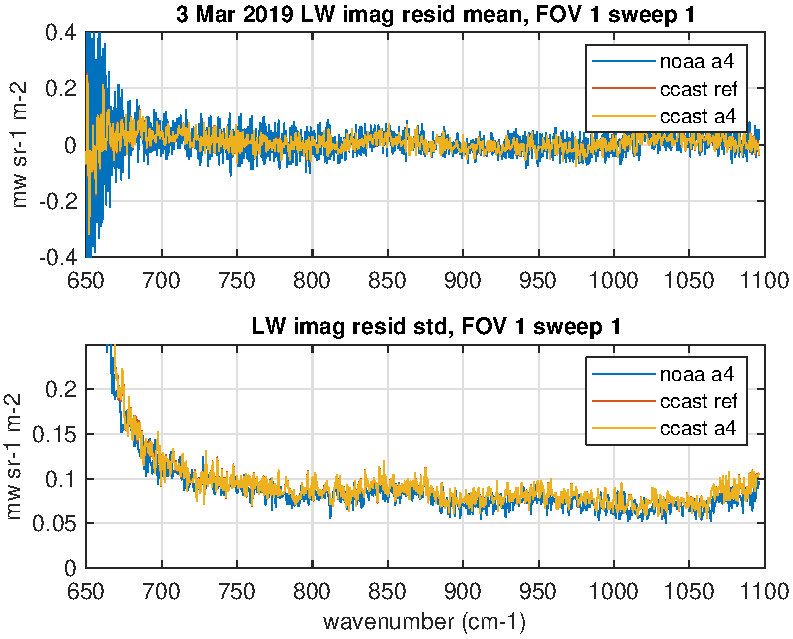
\includegraphics[width=\textwidth]{figures/LW_pre_fail_imag_fov1_sd1.pdf}
  \end{centering}\vspace{3mm}
  Pre-anomaly complex residual mean and standard deviation.  The NOAA complex
  residual is slightly larger.

\end{column}
\begin{column}{0.5\textwidth}  
  \begin{centering}
  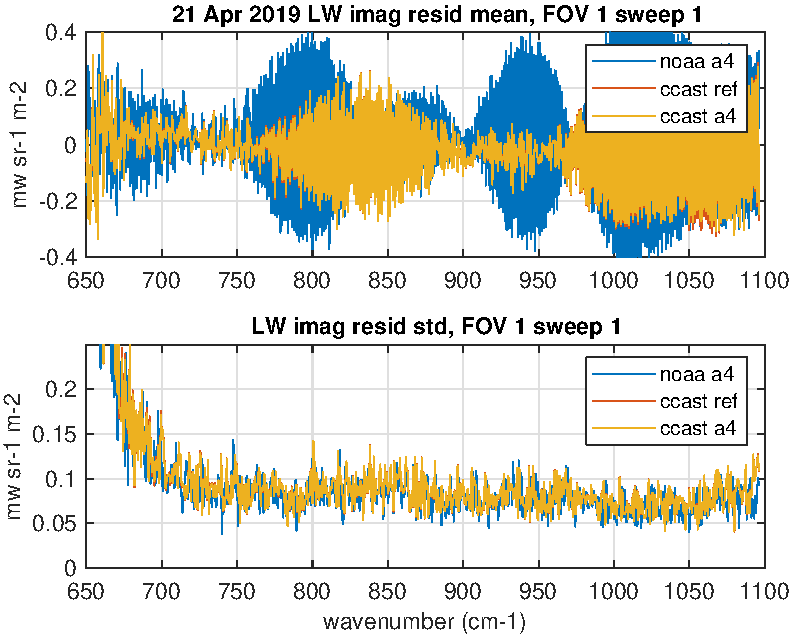
\includegraphics[width=\textwidth]{figures/LW_post_fail_imag_fov1_sd1.pdf}
  \end{centering}\vspace{3mm}
  Post-anomaly complex residual mean and standard deviation.  \\The
  NOAA complex residual is significantly larger.

\end{column}
\end{columns}
\end{frame}
%----------- slide --------------------------------------------------%
\begin{frame}
\frametitle{LW FOV 2 Sweep 1 Complex Residuals}
\begin{columns}[t]
\begin{column}{0.5\textwidth}
  \begin{centering}
  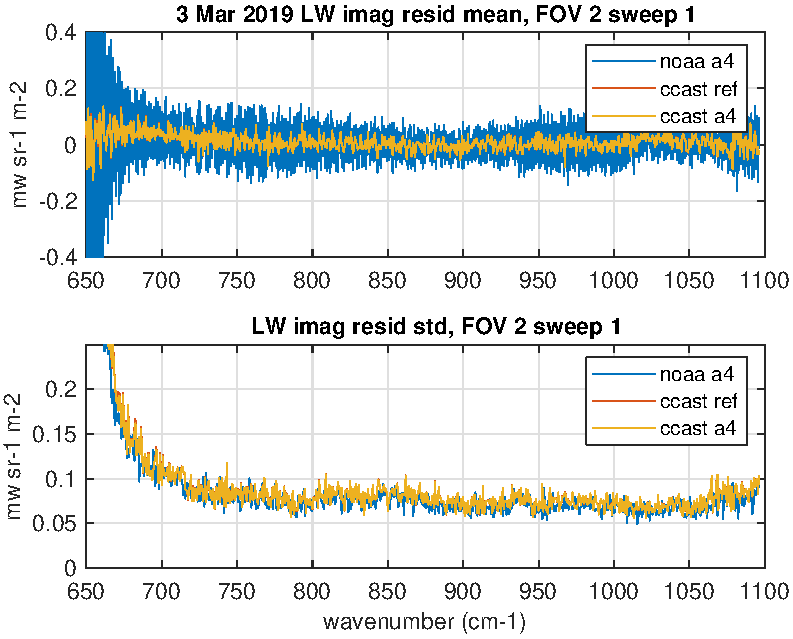
\includegraphics[width=\textwidth]{figures/LW_pre_fail_imag_fov2_sd1.pdf}
  \end{centering}\vspace{3mm}
  Pre-anomaly complex residual mean and standard deviation.  The
  NOAA complex residual is significantly larger.

\end{column}
\begin{column}{0.5\textwidth}  
  \begin{centering}
  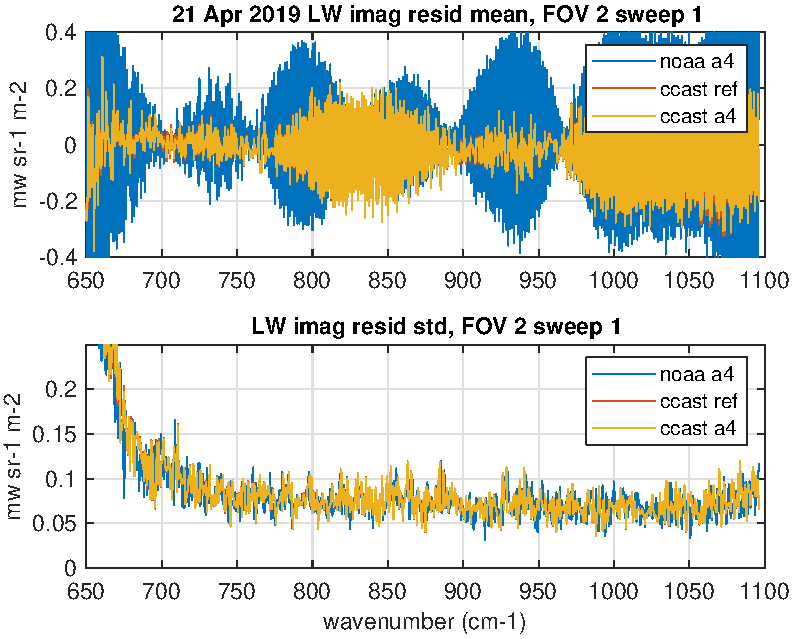
\includegraphics[width=\textwidth]{figures/LW_post_fail_imag_fov2_sd1.pdf}
  \end{centering}\vspace{3mm}
  Post-anomaly complex residual mean and standard deviation.  \\The
  NOAA complex residual is significantly larger.

\end{column}
\end{columns}
\end{frame}
%----------- slide --------------------------------------------------%
\begin{frame}
\frametitle{LW FOV 5 Sweep 1 Complex Residuals}
\begin{columns}[t]
\begin{column}{0.5\textwidth}
  \begin{centering}
  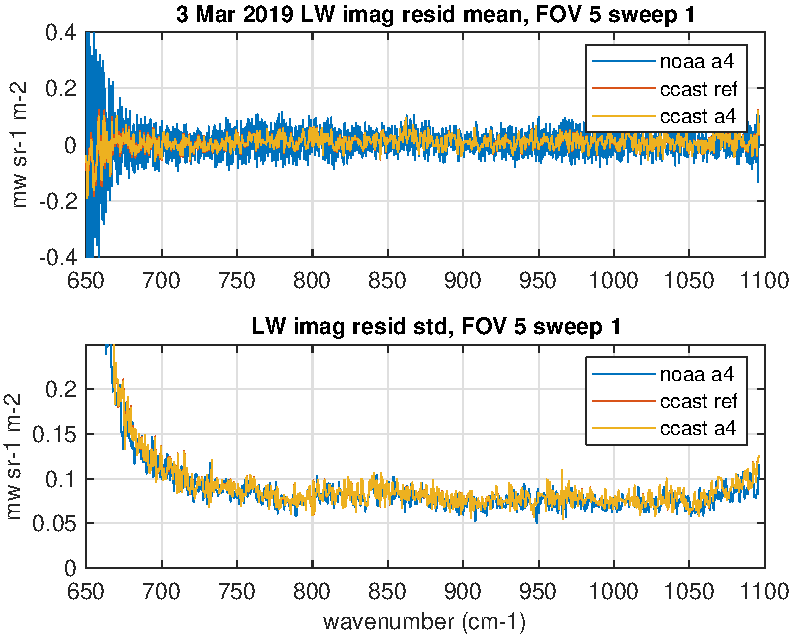
\includegraphics[width=\textwidth]{figures/LW_pre_fail_imag_fov5_sd1.pdf}
  \end{centering}\vspace{3mm}
  Pre-anomaly complex residual mean and standard deviation.  The NOAA complex
  residual is slightly larger.

\end{column}
\begin{column}{0.5\textwidth}  
  \begin{centering}
  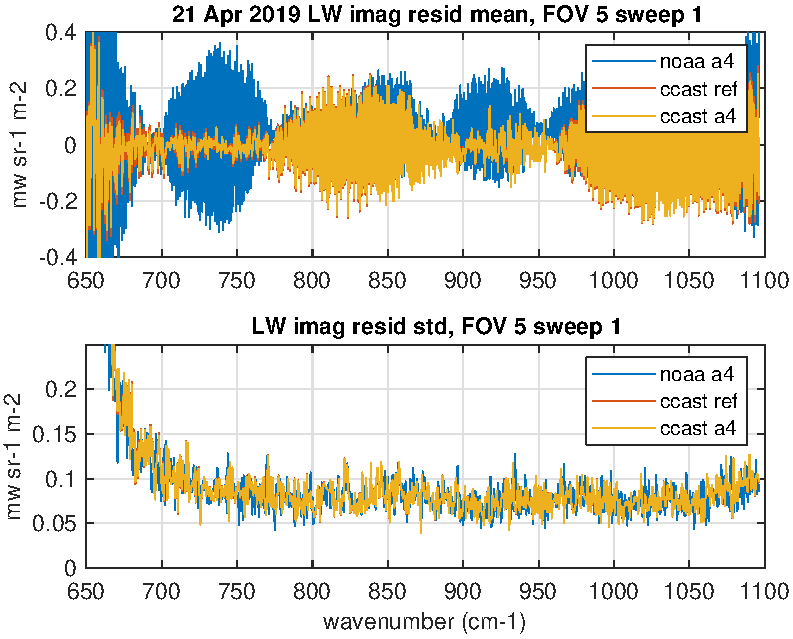
\includegraphics[width=\textwidth]{figures/LW_post_fail_imag_fov5_sd1.pdf}
  \end{centering}\vspace{3mm}
  Post-anomaly complex residual mean and standard deviation.  The
  NOAA residual is generally larger.

\end{column}
\end{columns}
\end{frame}
%----------- slide --------------------------------------------------%
\begin{frame}
\frametitle{LW FOV 1 Sweep 1 BT Spectra}
\begin{columns}[t]
\begin{column}{0.5\textwidth}
  \begin{centering}
  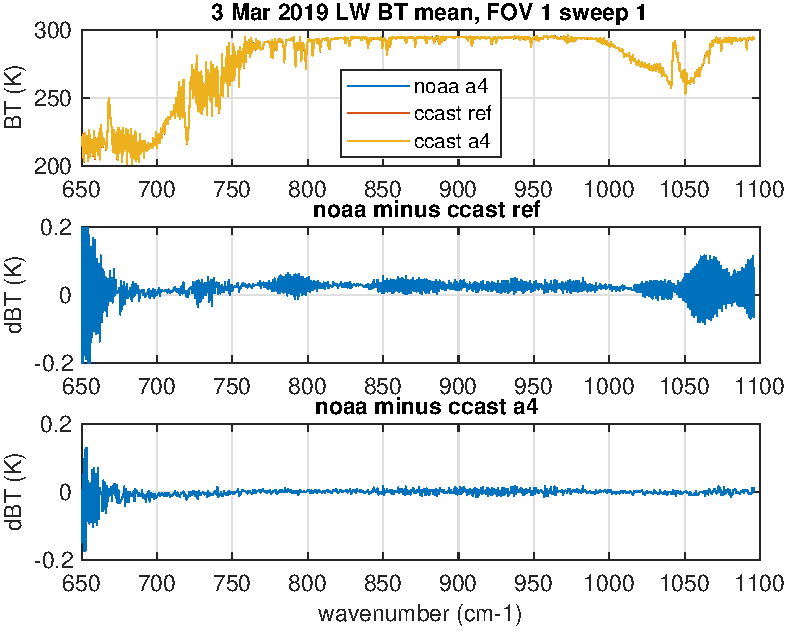
\includegraphics[width=\textwidth]{figures/LW_pre_fail_BT_fov1_sd1.pdf}
  \end{centering}\vspace{3mm}
  Pre-anomaly mean BT spectra for NOAA A4, CCAST ref, and CCAST A4.
  The CCAST A4 and NOAA A4 algorithms are in good agreement.

\end{column}
\begin{column}{0.5\textwidth}  
  \begin{centering}
  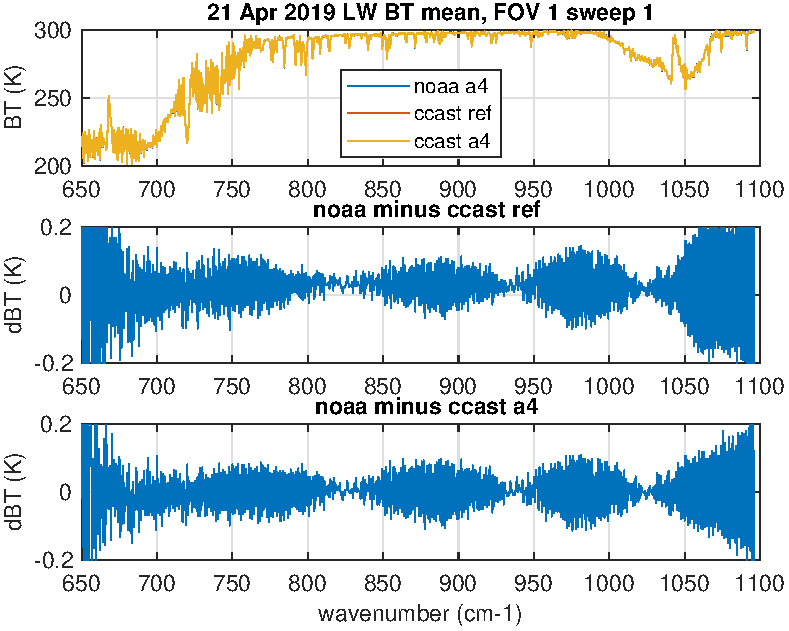
\includegraphics[width=\textwidth]{figures/LW_post_fail_BT_fov1_sd1.pdf}
  \end{centering}\vspace{3mm}
  Post-anomaly mean BT spectra for NOAA A4, CCAST ref, and CCAST A4.
  The differences suggest high frequency components with different
  periods, that is.

\end{column}
\end{columns}
\end{frame}
%----------- slide --------------------------------------------------%
\begin{frame}
\frametitle{LW FOV 1 Sweep 1 Sarta Residuals}
\begin{columns}[t]
\begin{column}{0.5\textwidth}
  \begin{centering}
  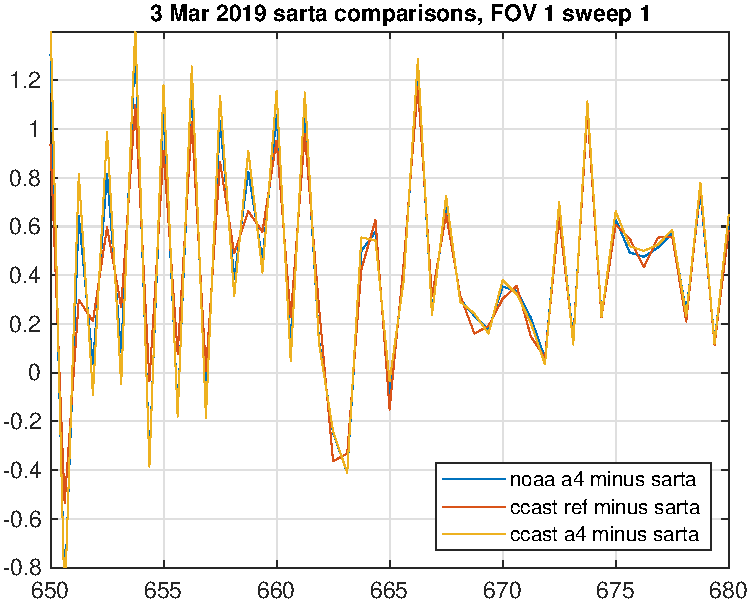
\includegraphics[width=\textwidth]{figures/LW_pre_fail_sarta_fov1_sd1.pdf}
  \end{centering}\vspace{3mm}
  Pre-anomaly mean BT spectra for NOAA A4, CCAST ref, and CCAST A4.
  The CCAST A4 and NOAA A4 algorithms are in good agreement.

\end{column}
\begin{column}{0.5\textwidth}  
  \begin{centering}
  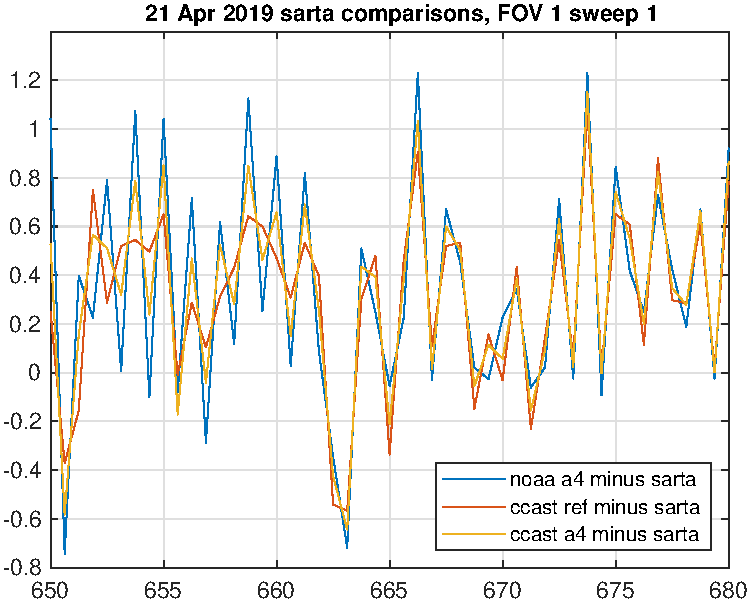
\includegraphics[width=\textwidth]{figures/LW_post_fail_sarta_fov1_sd1.pdf}
  \end{centering}\vspace{3mm}
  Post-anomaly mean BT spectra for NOAA A4, CCAST ref, and CCAST A4.
  The differences suggest high frequency components with different
  periods, that is.

\end{column}
\end{columns}
\end{frame}
%----------- slide --------------------------------------------------%
\begin{frame}
\frametitle{LW FOV 2 Sweep 1 BT Spectra}
\begin{columns}[t]
\begin{column}{0.5\textwidth}
  \begin{centering}
  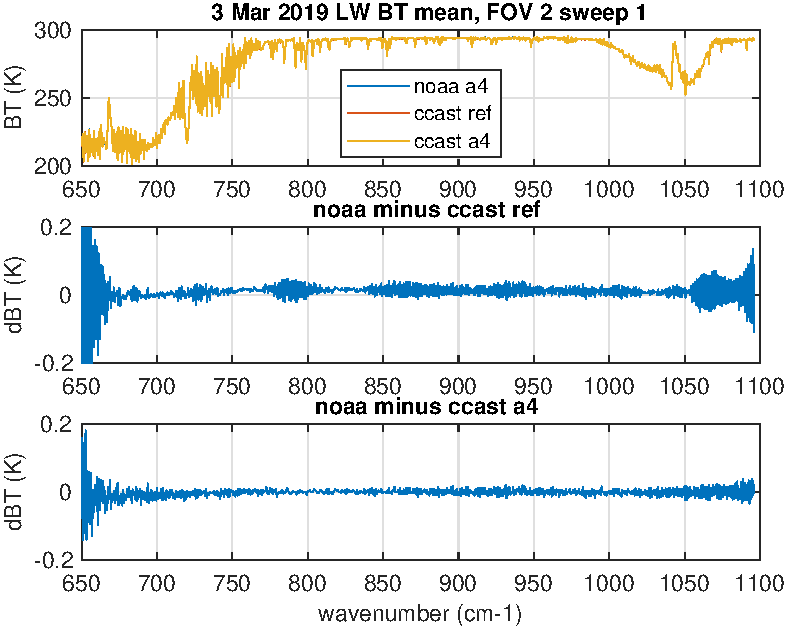
\includegraphics[width=\textwidth]{figures/LW_pre_fail_BT_fov2_sd1.pdf}
  \end{centering}\vspace{3mm}
  Pre-anomaly mean BT spectra.  \\The CCAST A4 and NOAA A4 algorithms
  are in good agreement.

\end{column}
\begin{column}{0.5\textwidth}  
  \begin{centering}
  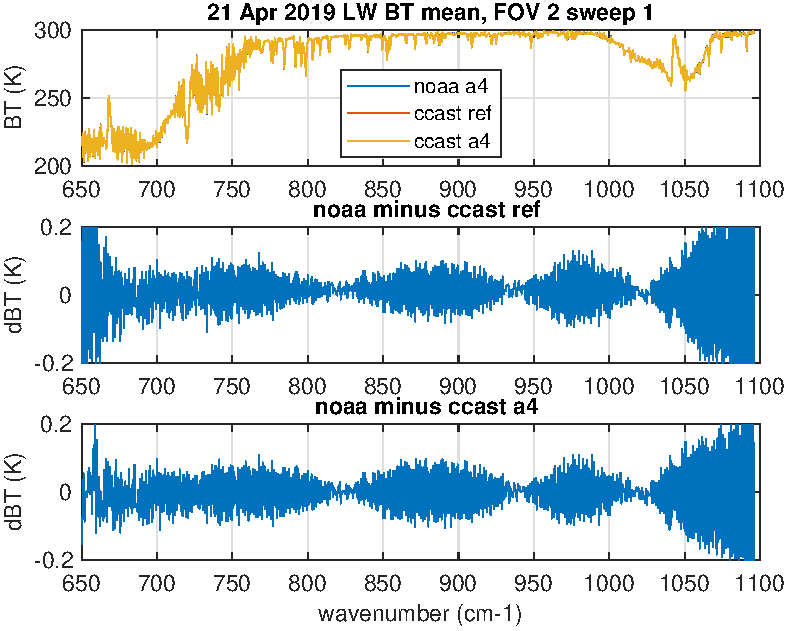
\includegraphics[width=\textwidth]{figures/LW_post_fail_BT_fov2_sd1.pdf}
  \end{centering}\vspace{3mm}
  Post-anomaly mean BT spectra. The differences suggest high
  frequency components with different periods, that is, different
  ringing.

\end{column}
\end{columns}
\end{frame}
%----------- slide --------------------------------------------------%
\begin{frame}
\frametitle{LW FOV 2 Sweep 1 Sarta Residuals}
\begin{columns}[t]
\begin{column}{0.5\textwidth}
  \begin{centering}
  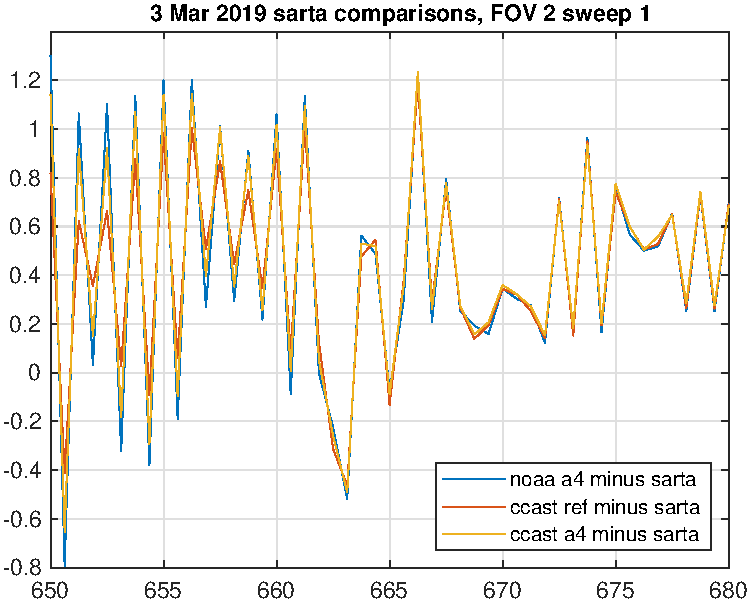
\includegraphics[width=\textwidth]{figures/LW_pre_fail_sarta_fov2_sd1.pdf}
  \end{centering}\vspace{3mm}
  Pre-anomaly mean BT spectra.  \\The CCAST A4 and NOAA A4 algorithms
  are in good agreement.

\end{column}
\begin{column}{0.5\textwidth}  
  \begin{centering}
  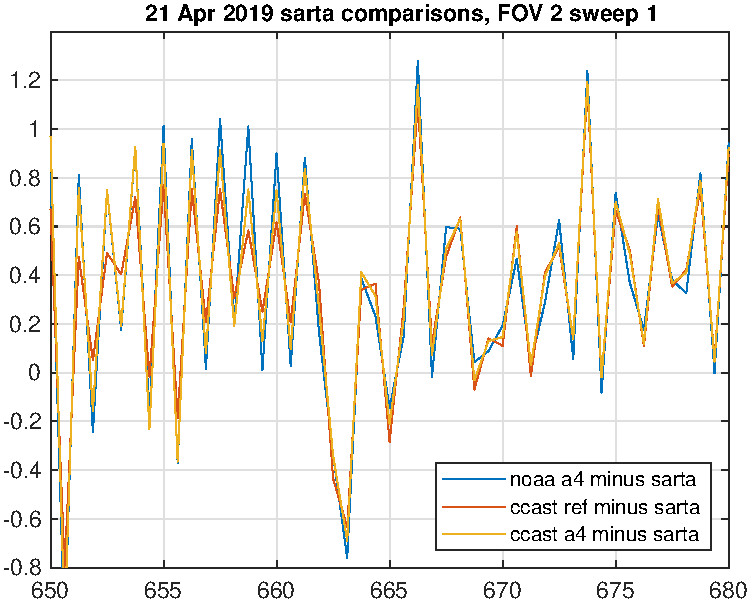
\includegraphics[width=\textwidth]{figures/LW_post_fail_sarta_fov2_sd1.pdf}
  \end{centering}\vspace{3mm}
  Post-anomaly mean BT spectra. The differences suggest high
  frequency components with different periods, that is, different
  ringing.

\end{column}
\end{columns}
\end{frame}
%----------- slide --------------------------------------------------%
\begin{frame}
\frametitle{LW FOV 5 Sweep 1 BT Spectra}
\begin{columns}[t]
\begin{column}{0.5\textwidth}
  \begin{centering}
  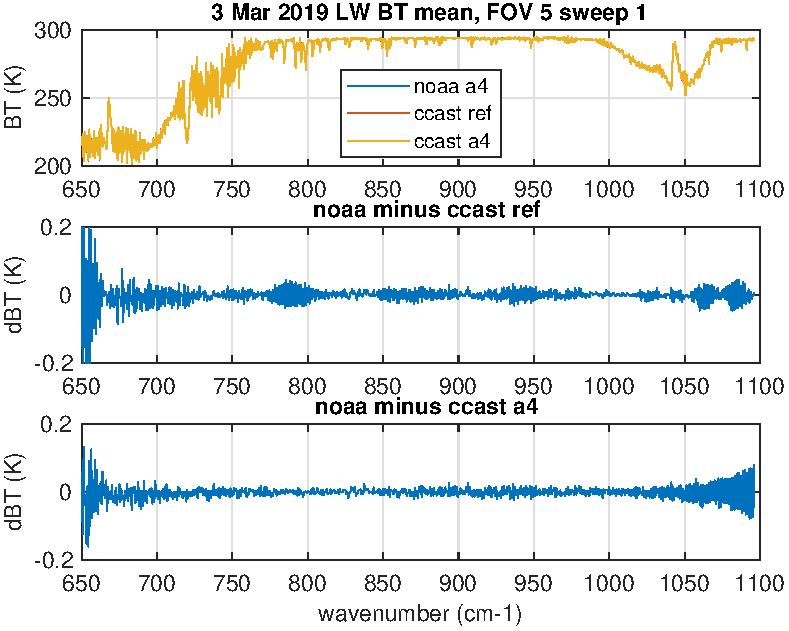
\includegraphics[width=\textwidth]{figures/LW_pre_fail_BT_fov5_sd1.pdf}
  \end{centering}\vspace{3mm}
  Pre-anomaly mean BT spectra.  \\The CCAST and NOAA algorithms are
  in relatively good agreement.

\end{column}
\begin{column}{0.5\textwidth}  
  \begin{centering}
  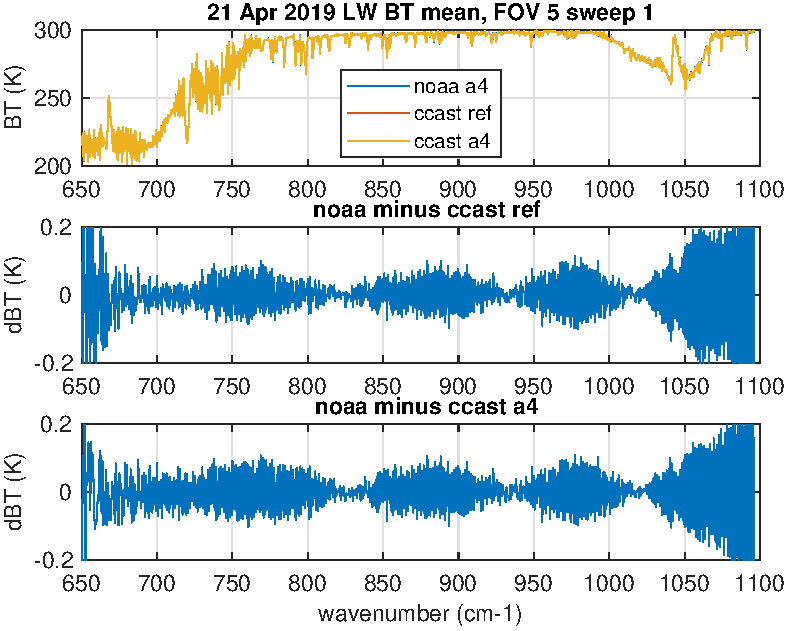
\includegraphics[width=\textwidth]{figures/LW_post_fail_BT_fov5_sd1.pdf}
  \end{centering}\vspace{3mm}
  Post-anomaly mean BT spectra.  The differences suggest high
  frequency components with different periods.

\end{column}
\end{columns}
\end{frame}
%----------- slide --------------------------------------------------%
\begin{frame}
\frametitle{LW FOV 5 Sweep 1 Sarta Residuals}
\begin{columns}[t]
\begin{column}{0.5\textwidth}
  \begin{centering}
  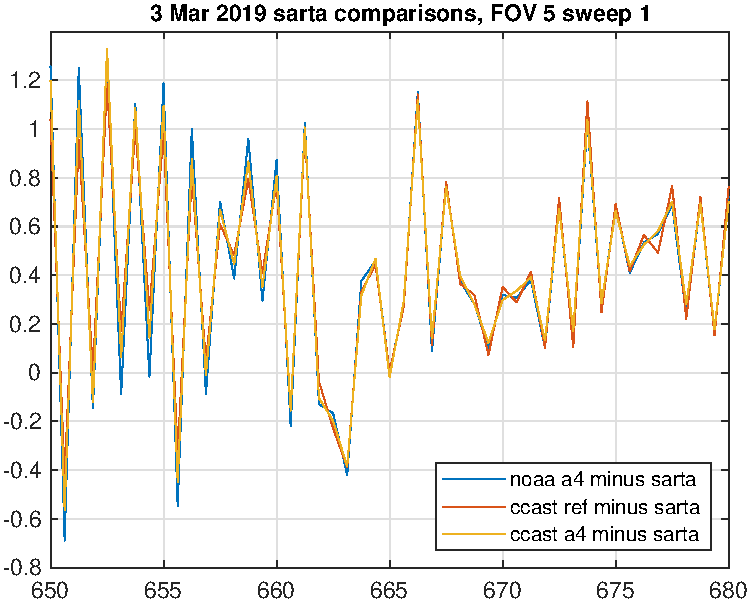
\includegraphics[width=\textwidth]{figures/LW_pre_fail_sarta_fov5_sd1.pdf}
  \end{centering}\vspace{3mm}
  Pre-anomaly mean BT spectra.  \\The CCAST and NOAA algorithms are
  in relatively good agreement.

\end{column}
\begin{column}{0.5\textwidth}  
  \begin{centering}
  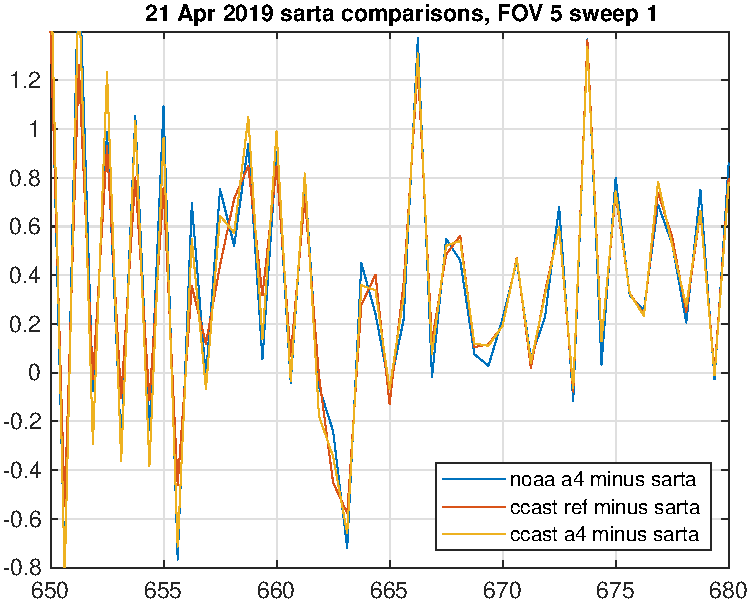
\includegraphics[width=\textwidth]{figures/LW_post_fail_sarta_fov5_sd1.pdf}
  \end{centering}\vspace{3mm}
  Post-anomaly mean BT spectra.  The differences suggest high
  frequency components with different periods.

\end{column}
\end{columns}
\end{frame}
%----------- slide --------------------------------------------------%
\begin{frame}
\frametitle{Conclusions}
\begin{itemize}

  \item Complex residuals for the NOAA product are slightly larger
    before and significanty larger after the anomaly.

  \item This may be due to the mild cosine apodization working
    better for the case of a significant ZPD shift.

  \item Because the complex residuals are smaller, we suspect
    the CCAST BT spectra are closer to reference truth after the
    anomaly.  But this needs to be verified.

  \item The slightly larger NOAA complex residuals before the
    anomaly are puzzling, we do not recall seeing this in earlier
    tests.

  \item The CCAST complex residual standard deviation is larger
    than NOAA for the SW side and corner FOVs.  This may be due to
    the different forms of the SA matrix.

  \item The next step is comparison with calculated reference truth,
    from clear matchups.

\end{itemize}
\end{frame}
%----------- slide --------------------------------------------------%

\end{document}

